{}\documentclass[letterpaper,
compress,
xcolor=x11names,
%draft,
]{beamer}
% Package imports
\usepackage{mathtools} % imports `amsmath'
\DeclareMathOperator{\sech}{sech}
\usepackage{amssymb}
\usepackage{fixltx2e}
\usepackage{lmodern}
\usepackage{movie15}
%\usepackage{media9}
\usepackage{microtype}
\usepackage{animate}
\usepackage{subcaption}
\captionsetup{compatibility=false}

% I just did this
\usepackage[english]{babel}
\usepackage[utf8]{inputenc}
\usepackage{amsmath}
\usepackage{graphicx}
\usepackage[colorinlistoftodos]{todonotes}
\usepackage{tikz}
\usetikzlibrary{tikzmark}
\usepackage{array}
\usepackage{layout}
\usepackage{multicol}
\usepackage{multirow}
\usepackage{booktabs}
%I just did this

% `beamer' configuration
\usefonttheme{professionalfonts}
\useoutertheme[subsection=false,]{miniframes}
\setbeamercolor*{alerted text}{fg=red}
\setbeamercolor*{example text}{fg=black}
\definecolor{CSU_green}{RGB}{30, 70, 43}
\definecolor{CSU_gold}{RGB}{200, 195, 114}
\setbeamercolor*{lower separation line head}{bg=CSU_gold}
\setbeamercolor*{section in head/foot}{fg=white,bg=CSU_green}
\setbeamercolor*{subsection in head/foot}{bg=white}
\setbeamercolor*{upper separation line head}{bg=CSU_gold}
\setbeamercolor*{page number in head/foot}{fg=CSU_green}
\setbeamercolor*{normal text}{fg=black,bg=white}
\setbeamercolor*{palette tertiary}{fg=black,bg=black!10}
\setbeamercolor*{palette quaternary}{fg=black,bg=black!10}
\setbeamercolor*{structure}{fg=black}
\setbeamerfont{frametitle}{shape=\scshape}
\setbeamerfont{institute}{shape=\scshape}
\setbeamerfont{section in head/foot}{shape=\scshape}
\setbeamerfont{subsection in head/foot}{shape=\scshape}
\setbeamertemplate{bibliography item}{}
\setbeamertemplate{itemize items}[ball]
\setbeamertemplate{navigation symbols}{}
\setbeamertemplate{footline}[frame number]
\usetikzlibrary{calc,arrows}
\graphicspath{{graphics/}{graphics/movies/}{graphics/images/}}
\usepackage{remreset}                  % hack to display beamer navigation
\makeatletter                          % circles even if not declaring
\@removefromreset{subsection}{section} % subsections
\makeatother                           % see: http://tex.stackexchange.com/a/2078
\setcounter{subsection}{1}             % see: https://bitbucket.org/rivanvx/beamer/issue/218

% `biblatex' configuration
\usepackage[backend=biber,
style=authortitle-comp,
]{biblatex}
\addbibresource{presentation.bib}

% `enumitem' configuration
\usepackage{enumitem}
\setlist[itemize,1]{label=\usebeamertemplate{itemize item}}
\setlist[itemize,2]{label=\usebeamertemplate{itemize subitem}}
\setlist[itemize,3]{label=\usebeamertemplate{itemize subsubitem}}
\DeclareMathOperator{\sinc}{sinc}


% `graphicx' configuration
\usepackage{graphicx}
\begin{document}
	\title{Nonlinear Solvers}
	%\subtitle{MATH-151:  Mathematical Algorithms in Matlab}
	\author{MATH-151:  Mathematical Algorithms in Matlab}
	\date[202X]{October 9, 2023}
	\titlegraphic{
\includegraphics[height = 3cm]{CSU_Ram_Logo.jpg}}



%%%%%%%%%%%%%%%%%%%%%%%%%%%%%%%%%%%%%%%%%%%%%%%%%%%%%%

\begin{frame}
\titlepage
\end{frame}
%%%%%%%%%%%%%%%%%%%%%%%%%%%%%%%%%%%%%%%%%%%%%%%%%%%%%%%%%
\section{Nonlinear Equations}

\begin{frame}{Why Solve Nonlinear Equations?}
	\footnotesize
	\begin{itemize}
		\item We are going to focus now on finding $x$ for a function such that $f(x) = 0$
		\item Lines are great, we know how to solve for where a line crosses zero quite easily, but many things in real life are nonlinear so we need to develop techniques for finding zeros for those equations as well
		\item<2-> Why do we want to find zeros in the first place?
		\begin{itemize}
			\item<3-> If we know how to find where $f(x)=0$, we know how to find where it is any other $c$ since we can instead solve $f(x) - c = g(x) = 0$
			\item<3-> If we want to find where two curves $f(x)$ and $g(x)$ intersect, we can do $f(x) - g(x) = h(x) = 0$
			\item<3-> Most engineering problems are interested in optimization. We remember from Calc I, if we want to find a minimizer or maxmizer, we start by finding a critical point where $f'(x) = 0$
		\end{itemize}
		\item<4-> Basically any time we want to know where anything occurs, we either run into a line or a case to solve for the root of a nonlinear equation!
		\begin{itemize}
			\item We usually like to know when/where things occur
		\end{itemize}
	\end{itemize}
\end{frame}


%%%%%%%%%%%%%%%%%%%%%%%%%%%%%%%%%%%%%%%%%%%%%%%%%%%%%%%%%

\begin{frame}{Bisection Method}
	\footnotesize
	\begin{itemize}
		\item We've already seen one of these a few weeks ago! The Bisection method!
		\item<2-> Suppose we know $f(a)$ is negative and $f(b)$ is positive. If $f$ is a continuous function, it must pass through 0 between $a$ and $b$.
		\item<3-> So we cut it in half and try $f(m)$, where $m  =\frac{a+b}{2}$
		\begin{itemize}
			\item If it has the same sign as $f(a)$, $m$ becomes our new $a$
			\item If it has the same sign as $f(b)$, $m$ becomes our new $b$
		\end{itemize} 
		\onslide<3->{
			\begin{center}
				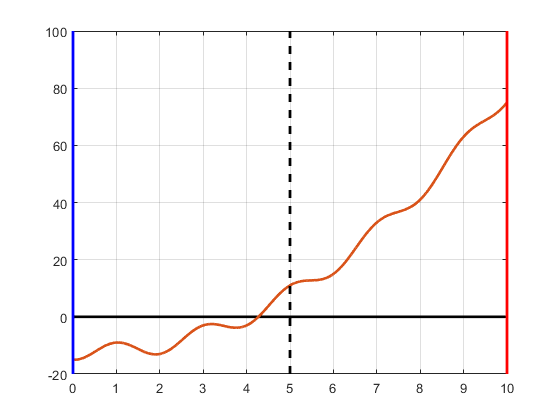
\includegraphics[width = 3cm]{bisection_1.png} \hspace{0.25cm}
				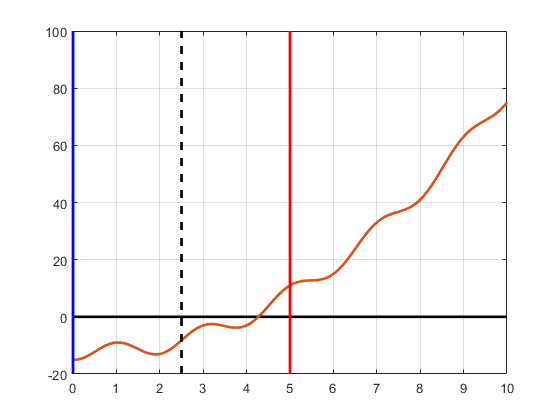
\includegraphics[width = 3cm]{bisection_2.png} \hspace{0.25cm}
				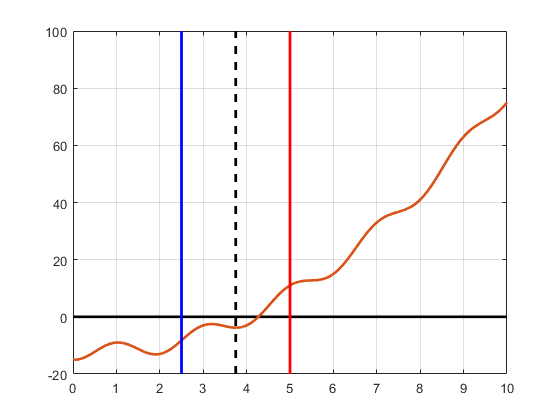
\includegraphics[width = 3cm]{bisection_3.png}
		\end{center}}
		\item<4-> This gives us a new, smaller possible range, so we do Bisection Method on that range
		\item<4-> We continue until $f(m)$ is sufficiently small.
	\end{itemize}
\end{frame}

%%%%%%%%%%%%%%%%%%%%%%%%%%%%%%%%%%%%%%%%%%%%%%%%%%%%%%%%%

\section{Fixed Point Methods}

\begin{frame}{Fixed Point Equations}
	\footnotesize
	\begin{itemize}
		\item How do we tell the computer to know when it's found a zero? For that we introduce the concept of a \textbf{fixed point}. 
		\item<2-> If $g(x)$ is a function that tells us our next guess for the zero, a fixed point satisfies the following
		\begin{equation*}
			x_n = g(x_n) = x_n + f(x_n)h(x_n)
		\end{equation*}
		\item<3-> When this occurs, our guess for the next point is the same as our current guess
		\begin{itemize}
			\item This will occur when $f(x_n) = 0$
		\end{itemize}
		\item<4-> That's what we are looking for! We found an $x_n$ such that $f(x_n)=0$.
		\begin{itemize}
			\item Remember, we will almost never get exactly 0 so we repeat our process until $f(x_n)$ or $x_n - x_{n-1}$ become small enough
			\item Or perhaps, we repeat \textit{while} $f(x_n)$ is too big
		\end{itemize}
		\item<5-> Great! So what can we do to set these up? What would this $g(x_n)$ look like?
	\end{itemize}
\end{frame}

%%%%%%%%%%%%%%%%%%%%%%%%%%%%%%%%%%%%%%%%%%%%%%%%%%%%%%%%%

\begin{frame}{Newton's Method}
	\footnotesize
	\begin{itemize}
		\item This is a widely used method that is usually much faster than bisection method!
		\item<2-> We pretend our function is the tangent line at our current guess, so that means our next guess for $x$ is where the tangent line crosses 0
		\begin{equation*}
			x_{n+1} = x_n - \frac{f(x_n)}{f'(x_n)}
		\end{equation*}
		\begin{center}
			\onslide<2->{
				\includegraphics[width = 3cm]{newton_1.png} \hspace{0.25cm}
				\includegraphics[width = 3cm]{newton_2.png} \hspace{0.25cm}
				\includegraphics[width = 3cm]{newton_3.png}
			}
		\end{center}
		\item<3-> We are not only using the values of our function, but also information about what the curve looks like. This will help us get closer to our 0 faster!
		\begin{itemize}
			\item This does have some risk though, we could encounter a point where $f'(x_n) = 0$...
		\end{itemize}
	\end{itemize}
\end{frame}

%%%%%%%%%%%%%%%%%%%%%%%%%%%%%%%%%%%%%%%%%%%%%%%%%%%%%%%%%

\begin{frame}{Secant Method}
	\footnotesize
	\begin{itemize}
		\item Sometimes we don't have a derivative function, or it would be very difficult to implement 
		\item<2-> In those cases, we can estimate our derivative using finite difference method with our last 2 points!
		\begin{itemize}
			\item But this means we need to make 2 initial guesses to start
		\end{itemize}
		\item<3-> Doing this we have a slightly different method called \textbf{Secant Method}
		\begin{equation*}
			x_{n+1} = x_n - f(x_n)\frac{x_n - x_{n-1}}{f(x_n) - f(x_{n-1})}
		\end{equation*}
		\onslide<3->{
		\begin{center}
			\includegraphics[width = 3cm]{secant_1.png} \hspace{0.25cm}
			\includegraphics[width = 3cm]{secant_2.png} \hspace{0.25cm}
			\includegraphics[width = 3cm]{secant_3.png}
		\end{center}
		}
		\item<4-> The code I use in my research is actually using Secant method because our gradients are too complicated to find analytically!
	\end{itemize}
\end{frame}
\end{document}